\documentclass{article}
\usepackage[utf8]{inputenc}

\title{EEC-201 Final Project}
\author{Igor Sheremet and Jonathan Tivald }
\date{March 2021}

\usepackage{natbib}
\usepackage{graphicx}
\usepackage{listings}
\usepackage{xcolor}
\usepackage{float}
\usepackage{enumitem}
\usepackage{hyperref}

\definecolor{codegreen}{rgb}{0,0.6,0}
\definecolor{codegray}{rgb}{0.5,0.5,0.5}
\definecolor{codepurple}{rgb}{0.58,0,0.82}
\definecolor{backcolour}{rgb}{0.95,0.95,0.92}

\lstdefinestyle{mystyle}{
    backgroundcolor=\color{backcolour},   
    commentstyle=\color{codegreen},
    keywordstyle=\color{magenta},
    numberstyle=\tiny\color{codegray},
    stringstyle=\color{codepurple},
    basicstyle=\ttfamily\footnotesize,
    breakatwhitespace=false,         
    breaklines=true,                 
    captionpos=b,                    
    keepspaces=true,                 
    numbers=left,                    
    numbersep=5pt,                  
    showspaces=false,                
    showstringspaces=false,
    showtabs=false,                  
    tabsize=2
}

\lstset{style=mystyle}

\begin{document}

\maketitle

\section{Speech Data Files}
Down load the ZIP file of the speech database from canvas. After unzipping the file, you will 11 speech
files, named: S1.WAV, S2.WAV, …; each is labeled after the ID of the speaker. These files were recorded
in WAV format.\\
Our goal is to train a voice model (e.g., a VQ codebook in the MFCC vector space) for each speaker using
the corresponding sound file. After this training step, the system would have knowledge of the voice
characteristic of each (known) speaker. Next, in the testing phase, you should add noises to distort the
existing training signals to generate a test set. The amount of noises would vary to test the robustness of
your system.

\subsection{Test 1}
Play each sound file in the TRAIN folder. Can you distinguish the voices of the 11 speakers in
the database? Next play each sound in the TEST folder in a random order without looking at the
groundtruth and try to identify the speaker manually. Record what is your (human performance)
recognition rate. Use this result as a later benchmark.

\vspace{5mm} %5mm vertical space

    \begin{tabular}{ |p{3cm}|p{3cm}|p{3cm}|p{3cm}|  }
        \hline
        \multicolumn{3}{|c|}{Human Performance} \\
        \hline
        TEST Audio & Jonathan & Igor\\
        \hline
        s1& s1 & s\\
        s2& s2 & s\\
        s3& s3 & s\\
        s4& s4 & s\\
        s5& s5 & s\\
        s6& s6 & s\\
        s7& s7 & s\\
        s8& s8 & s\\
        \hline
    \end{tabular}

\section{Speech Processing}

\subsection{Test 2}
In Matlab one can play the sound file using “sound”. Record the sampling rate and compute how
many milliseconds of speech are contained in a block of 256 samples? \textbf{Now plot the signal to view it in
the time domain. It should be obvious that the raw data are long and may need to be normalized
because of different strengths.}

Use STFT to generate periodogram. Locate the region in the plot that contains most of the energy, in time
(msec) and frequency (in Hz) of the input speech signal. Try different frame size: for example N = 128, 256
and 512. In each case, set the frame increment M to be about N/3.

\subsection{Test 3}
Plot the mel-spaced filter bank responses. Compare them with theoretical responses. Compute
and plot the spectrum of a speech file before and after the mel-frequency wrapping step. Describe and
explain the impact of the melfb.m or melfbown.m program.

\subsection{Test 4}
Complete the “Cepstrum” step and put all pieces together into a single Matlab function, e.g.,
mfcc.m

\section{Vector Quantization}
Now apply VQ-based pattern recognition technique to build speaker reference models from those vectors in
the training set before identifying any sequences of acoustic vectors from unmarked speakers in the test set.

\subsection{Test 5}
To check whether the program is working, inspect the acoustic space (MFCC vectors) in any two
dimensions in a 2D plane to observe the results from different speakers. Are they in clusters?

Now write a function that trains a VQ codebook using the LGB algorithm.

\subsection{Test 6}
Plot the resulting VQ codewords using the same two dimensions over the plot of in TEST 5. You
should get a figure like Figure 4.

\section{Full Test and Demonstration}
Using the programs to train and test speaker recognition on the data sets.

\subsection{Test 7}
Record the results. What is recognition rate our system can perform? Compare this with human
performance. Experiment and find the reason if high error rate persists. Record more voices of yourself
and your teammates/friend. Each new speaker can provide one speech file for training and one for testing.
\textbf{Record the results.}

\subsection{Test 8}
Use notch filters on the voice signals to generate another test set. Test your system on the
accuracy after voice signals have passed different notch filters that may have suppressed distinct features of
the original voice signal. Report the robustness of your system.

\subsection{Test 9}
Test the system with other speech files you may find online. E.g.
\url{https://lionbridge.ai/datasets/best-speech-recognition-datasets-for-machine-learning/}

\section{LaTex Reference (temp)}

\begin{lstlisting}[language=Matlab]
    %
    %EEC-201, Winter Quarter 2021, Final Project
    %
    %Title: Speaker Recognition
    %
    %Description: This is main function of the final project for EEC-201.
    %             This program will store features in the recorded audio of 
    %             different speakers in order to recognize which speaker is
    %             talking on further recordings.
    %
    %Authors: Igor Sheremet and Jonathan Tivald
    %
    %Date: 2/7/2021
    
    clear all;
    close all;
    clc;
\end{lstlisting}

\begin{figure}[H]
\centering
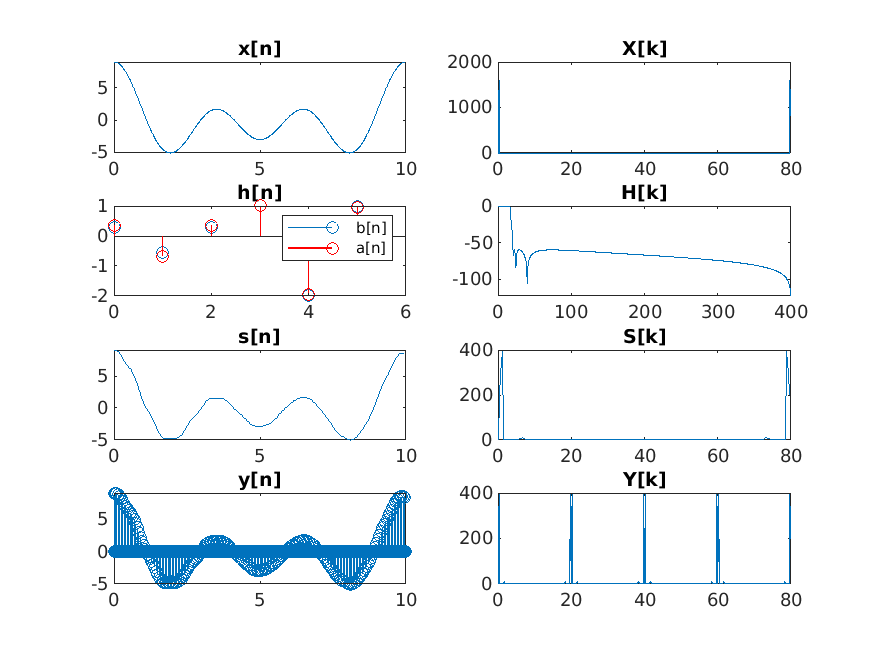
\includegraphics[scale=0.9]{problem1.png}
\end{figure}

\begin{enumerate}[label=(\alph*)]
    \item DC gain of g[n] is 0.2
    \item The zeros of G(z) = -1/(zeros of H(z))
    \item $abs(G(w)) = abs(H(w-pi))$
\end{enumerate}

\end{document}
